% !TEX root = ../FundationsDataScience.tex

%%%%%%%%%%%%%%%%%%%%%%%%%%%%%%%%%%%%%%%%%%%%%%%%%%%%%%%%%%%%%%%%%%%%%%%%
%%%%%%%%%%%%%%%%%%%%%%%%%%%%%%%%%%%%%%%%%%%%%%%%%%%%%%%%%%%%%%%%%%%%%%%%
%%%%%%%%%%%%%%%%%%%%%%%%%%%%%%%%%%%%%%%%%%%%%%%%%%%%%%%%%%%%%%%%%%%%%%%%
\section{Stochastic Optimization}
\label{sec-stochastic-optim}

We detail some important stochastic Gradient Descent methods, which enable to perform optimization in the setting where the number of samples $n$ is large and even infinite. 

% We set the classes indexes to be $\{-1,+1\}$, and remove empty features, normalize $X$. $n$ is the number of samples, $p$ is the dimensionality of the features,

%%%%%%%%%%%%%%%%%%%%%%%%%%%%%%%%%%%%%%%%%%%%%%%%%%%%%%%%
\subsection{Minimizing Sums and Expectation}

A large class of functionals in machine learning can be expressed as minimizing large sums of the form
\eql{\label{eq-min-sums}
	\umin{x \in \RR^p} f(x) \eqdef \frac{1}{n} \sum_{i=1}^n f_i(x)
}
or even expectations of the form
\eql{\label{eq-min-int}
	\umin{x \in \RR^p}  f(x) \eqdef \EE_{\zp \sim \pi}( f(x,\zp) ) = \int_{\Zz} f(x,z) \d\pi(z).
}
Problem~\eqref{eq-min-sums} can be seen as a special case of~\eqref{eq-min-int}, when using a discrete empirical uniform measure $\pi = \sum_{i=1}^n \de_i$ and setting $f(x,i)=f_i(x)$. One can also viewed~\eqref{eq-min-sums} as a discretized ``empirical'' version of~\eqref{eq-min-int} when drawing $(z_i)_i$ i.i.d. according to $\zp$ and defining $f_i(x)=f(x,z_i)$. In this setup,~\eqref{eq-min-sums} converges to~\eqref{eq-min-int} as $n \rightarrow +\infty$.

A typical example of such a class of problems is empirical risk minimization for linear model, where in these cases
\eql{\label{eq-stochastic-erm}
	f_i(x) = \ell(\dotp{a_i}{x},y_i)
	\qandq
	f(x,z) = \ell(\dotp{a}{x},y)
}
for $z=(a,y) \in \Zz = (\Aa=\RR^p) \times \Yy$ (typically $\Yy=\RR$ or $\Yy=\{-1,+1\}$ for regression and classification), where $\ell$ is some loss function. 
%
We illustrate bellow the methods on binary logistic classification, where
\eql{\label{eq-stoch-logistic}
	\loss(s,y) \eqdef \log( 1+\exp(-sy) ).
}
But this extends to arbitrary parametric models, and in particular deep neural networks.

While some algorithms (in particular batch gradient descent) are specific to finite sums~\eqref{eq-min-sums}, the stochastic methods we detail next work verbatim (with the same convergence guarantees) in the expectation case~\eqref{eq-min-int}. For the sake of simplicity, we however do the exposition for the finite sums case, which is sufficient in the vast majority of cases. But one should keep in mind that $n$ can be arbitrarily large, so it is not acceptable in this setting to use algorithms whose complexity per iteration depend on $n$.

If the functions $f_i(x)$ are very similar (the extreme case being that they are all equal), then of course there is a gain in using stochastic optimization (since in this case, $\nabla f_i \approx \nabla f$ but $\nabla f_i$ is $n$ times cheaper).
%
But in general stochastic optimization methods are not necessarily faster than batch gradient descent. 
%
If $n$ is not too large so that one afford the price of doing a few non-stochastic iterations, then deterministic methods can be faster.
%
But if $n$ is so large that one cannot do even a single deterministic iteration, then stochastic methods allow one to have a fine grained scheme by breaking the cost of determinstic iterations in smaller chunks. Another advantage is that they are quite easy to parallelize. 


%%%%%%%%%%%%%%%%%%%%%%%%%%%%%%%%%%%%%%%%%%%%%%%%%%%%%%%%
\subsection{Batch Gradient Descent (BGD)}

The usual deterministic (batch) gradient descent (BGD) is studied in details in Section~\ref{sec-grad-desc-basic}. Its iterations read
\eq{
	x_{k+1} = x_k - \tau_k \nabla f(x_k)
}
and the step size should be chosen as $0 < \tau_{\min} < \tau_k < \tau_{\max} \eqdef 2/L$ where $L$ is the Lipschitz constant of the gradient $\nabla f$. In particular, in this deterministic setting, this step size should not go to zero and this ensures quite fast convergence (even linear rates if $f$ is strongly convex).

The computation of the gradient in our setting reads
\eql{\label{eq-full-grad}
	\nabla f(x) = \frac{1}{n} \sum_{i=1}^n \nabla f_i(x)
}
so it typically has complexity $O(np)$ if computing $\nabla f_i$ has linear complexity in $p$.

For ERM-type functions of the form~\eqref{eq-stochastic-erm}, one can do the Taylor expansion of $f_i$
\begin{align*}
	f_i(x+\epsilon) &= \ell(\dotp{a_i}{x} + \dotp{a_i}{\epsilon},y_i)
	= \ell(\dotp{a_i}{x},y_i) + \ell'(\dotp{a_i}{x},y_i)\dotp{a_i}{\epsilon} + o(\norm{\epsilon}) \\
	&= f_i(x) + \dotp{\ell'(\dotp{a_i}{x},y_i) a_i}{x} + o(\norm{\epsilon}), 
\end{align*}
where $\ell( y,y' ) \in \RR$ is the derivative with respect to the first variable, i.e. the gradient of the map $y \in \RR \mapsto \loss(y,y') \in \RR$. This computation shows that 
\eql{\label{eq-grad-formula}
	\nabla f_i(x) =  \ell'( \dotp{a_i}{x},y_i ) a_i.
}
For the logistic loss, one has 
\eq{
	\loss'(s,y) = -s \frac{e^{-sy}}{ 1+e^{-sy} }.
}



\begin{figure}
\centering
\begin{tabular}{cc}
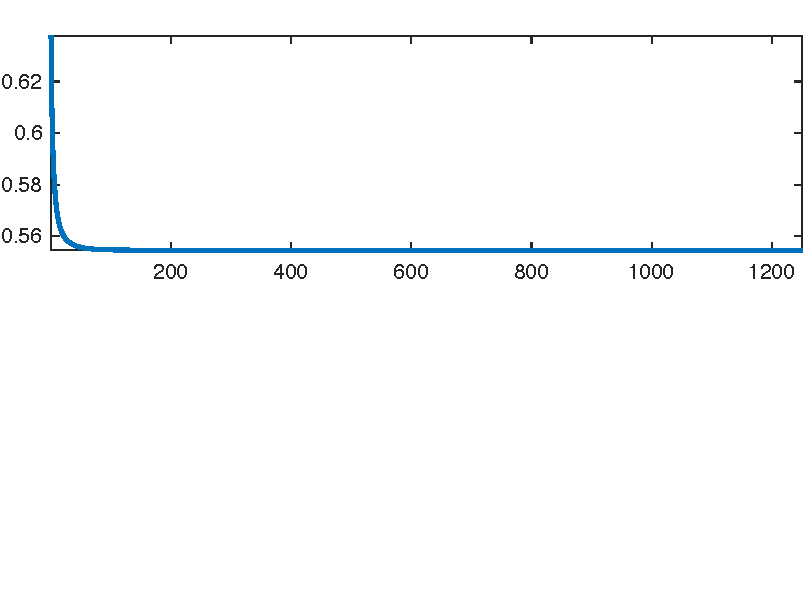
\includegraphics[width=.45\linewidth]{ml/sgd/error-bgd-1} &
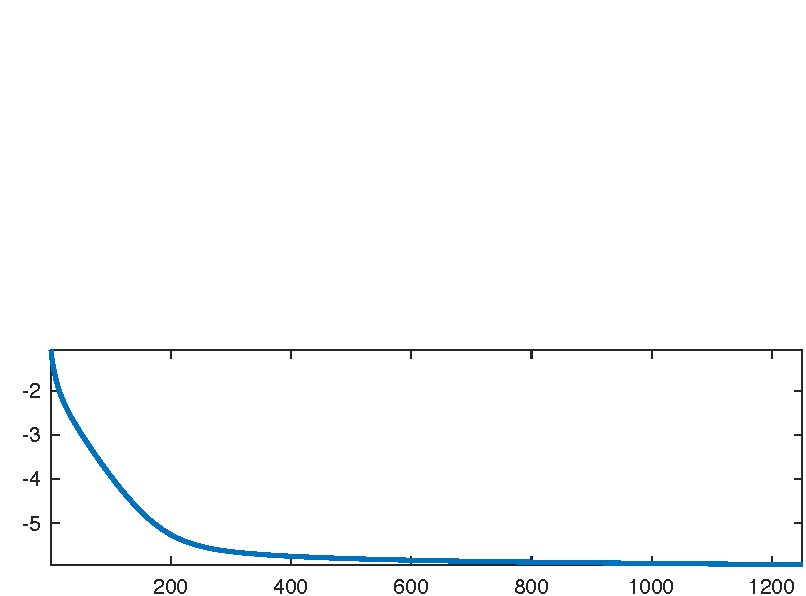
\includegraphics[width=.45\linewidth]{ml/sgd/error-bgd-2} \\
$f(x_k)$ & $\log_{10}(f(x_k)-f(x^\star))$ 
\end{tabular}
\caption{\label{fig-bgd}
Evolution of the error of the BGD for logistic classification.
}
\end{figure}



%%%%%%%%%%%%%%%%%%%%%%%%%%%%%%%%%%%%%%%%%%%%%%%%%%%%%%%%
\subsection{Stochastic Gradient Descent (SGD)}

\wrapf{ml/sgd/unbiased-grad}{Unbiased gradient estimate}
For very large $n$, computing the full gradient $\nabla f$ as in~\eqref{eq-full-grad} is prohibitive.  
%
The idea of SGD is to trade this exact full gradient by an inexact proxy using a single functional $f_{i}$ where $i$ is drawn uniformly at random. The main idea that makes this work is that this sampling scheme provides an unbiased estimate of the gradient, in the sense that
\eql{\label{eq-unbiased-grad}
	\EE_{\ip}{ \nabla f_{\ip}(x) } = \nabla f(x)
}
where $\ip$ is a random variable distributed uniformly in $\{1,\ldots,n\}$.

\wrapf{ml/sgd/sgd-schematic}{Schematic view of SGD iterates}
Starting from some $x_0$,the iterations of stochastic gradient descent (SGD) read
\eq{
	x_{k+1} = x_k - \tau_k \nabla f_{i(k)}(x_k)
}
where, for each iteration index $k$, $i(k)$
is drawn uniformly at random in $\{1,\ldots,n\}$. 
%
It is important that the iterates $x_{k+1}$ are thus random vectors, and the theoretical analysis of the method thus studies wether this sequence of random vectors converges (in expectation or in probability for instance) toward a deterministic vector (minimizing $f$), and at which speed. 

Note that each step of a batch gradient descent has complexity $O(np)$,
while a step of SGD only has complexity $O(p)$. SGD is thus
advantageous when $n$ is very large, and one cannot afford to do
several passes through the data. In some situation, SGD can provide
accurate results even with $k \ll n$, exploiting redundancy between
the samples.

A crucial question is the choice of step size schedule $\tau_k$. It
must tends to 0 in order to cancel the noise induced on the gradient by
the stochastic sampling. But it should not go too fast to zero in order
for the method to keep converging. 


A typical schedule that ensures both properties is to have asymptotically $\tau_k \sim k^{-1}$ for
$k\rightarrow +\infty$. We thus propose to use 
\eql{\label{eq-stepsize-sgd}
	\tau_k \eqdef \frac{\tau_0}{1 + k/k_0}
}
where $k_0$ indicates roughly the number of iterations serving as a
``warmup'' phase.

Figure~\ref{fig-sgd-traject} shows a simple 1-D example to minimize $f_1(x)+f_2(x)$ for $x \in \RR$ and $f_1(x)=(x-1)^2$ and $f_2(x)=(x+1)^2$. One can see how the density of the distribution of $x_k$ progressively clusters around the minimizer $x^\star=0$. Here the distribution of $x_0$ is uniform on $[-1/2,1/2]$.

\begin{figure}
\centering
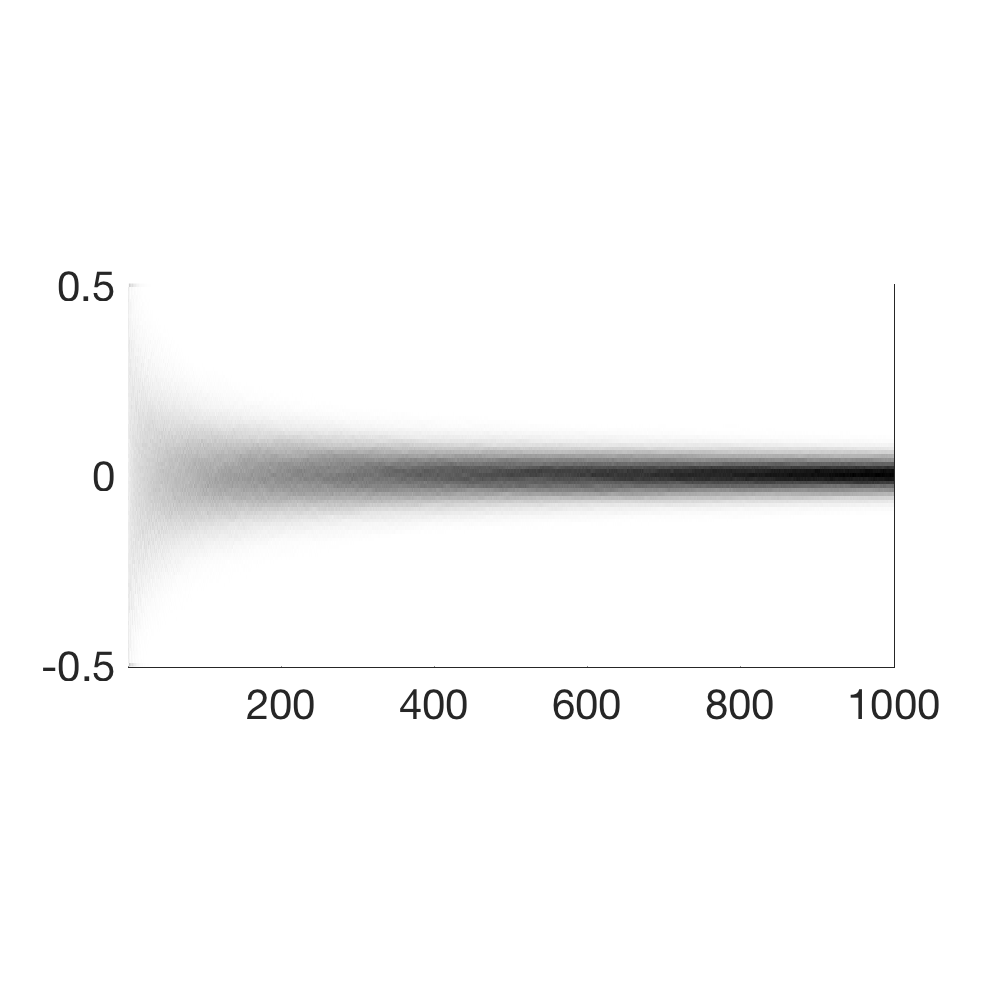
\includegraphics[width=.49\linewidth]{ml/sgd/sgd-histo} 
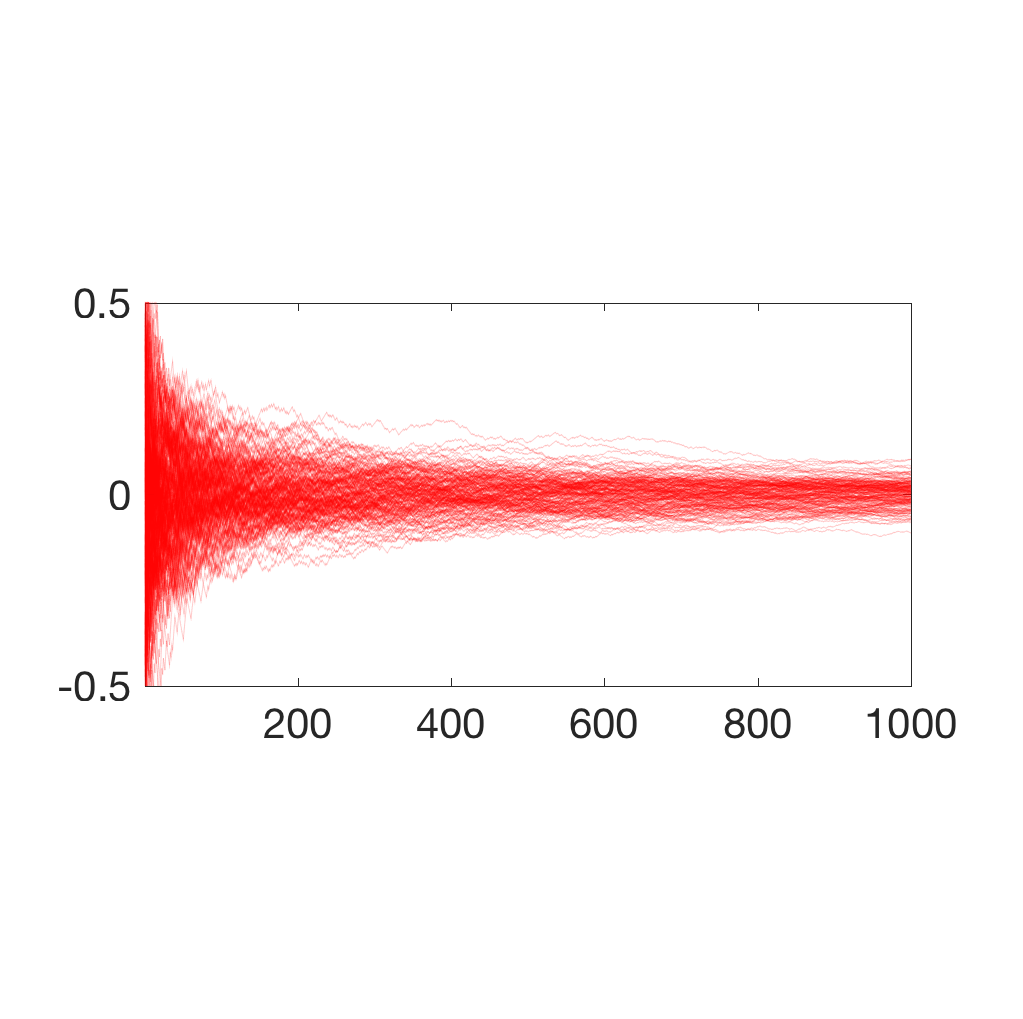
\includegraphics[width=.49\linewidth]{ml/sgd/sgd-trajectory}
\caption{\label{fig-sgd-traject}
Display of a large number of trajectories $k \mapsto x_k \in \RR$ generated by several runs of SGD. On the top row, each curve is a trajectory, and the bottom row displays the corresponding density.
}
\end{figure}

The following theorem shows the convergence in expectation with a $1/\sqrt{k}$ rate on the objective.

\begin{thm}\label{thm-conv-sgd}
We assume $f$ is $\mu$-strongly convex as defined in~\eqref{eq-strong-conv} (i.e. $\Id_{p}  \preceq \partial^2  f(x)$ if $f$ is $\Cc^2$), and is such that $\norm{\nabla f_i(x)}^2 \leq C^2$. 
For the step size choice $\tau_k = \frac{1}{\mu (k+1)}$, one has
\eql{\label{eq-rate-sgd}
	\EE( \norm{x_k-x^\star}^2 ) \leq \frac{ R }{k+1}
	\qwhereq
	 R = \max( \norm{x_0 - x^\star}, C^2/\mu^2 ), 
}
where $\EE$ indicates an expectation with respect to the i.i.d.
sampling performed at each iteration.
\end{thm}

\begin{proof}
	By strong convexity, one has
	\begin{align*}
		f(x^\star) - f(x_k) &\geq \dotp{ \nabla f(x_k) }{ x^\star-x_k } + \frac{\mu}{2}\norm{x_k-x^\star}^2 \\
		f(x_k) - f(x^\star) &\geq \dotp{ \nabla f(x^\star) }{ x_k - x^\star } + \frac{\mu}{2}\norm{x_k-x^\star}^2.
	\end{align*}
	Summing these two inequalities and using $\nabla f(x^\star)=0$ leads to
	\eql{\label{eq-sgd-proof-1}
		\dotp{ \nabla f(x_k) - \nabla f(x^\star) }{ x_k - x^\star }
		=
		\dotp{ \nabla f(x_k)  }{ x_k - x^\star }
		\geq \mu \norm{x_k-x^\star}^2.
	}
	Considering only the expectation with respect to the ransom sample of $i(k) \sim \ip_k$, one has
	\begin{align*}
		\EE_{\ip_k}( \norm{x_{k+1}-x^\star}^2 )
		&= 
		\EE_{\ip_k}( \norm{x_k - \tau_k \nabla f_{\ip_k}(x_k) -x^\star}^2 ) \\
		&= 
		\norm{x_k - x^\star}^2 + 2\tau_k \dotp{ \EE_{\ip_k}(\nabla f_{\ip_k}(x_k)) }{ x^\star - x_k  } + 
			\tau_k^2  \EE_{\ip_k}( \norm{\nabla f_{\ip_k}(x_k)}^2 ) \\
		&\leq
		\norm{x_k - x^\star}^2 + 2\tau_k \dotp{ \nabla f(x_k)) }{ x^\star - x_k  } + \tau_k^2 C^2 \\
	\end{align*}
	where we used the fact~\eqref{eq-unbiased-grad} that the gradient is unbiased. 
	%
	Taking now the full expectation with respect to all the other previous iterates, and using~\eqref{eq-sgd-proof-1} one obtains
	\eql{\label{eq-sgd-proof-2}
		\EE( \norm{x_{k+1}-x^\star}^2 ) \leq \EE( \norm{x_k - x^\star}^2 ) - 2 \mu \tau_k \EE( \norm{x_k - x^\star}^2 ) + \tau_k^2 C^2
		= (1-2 \mu \tau_k)  \EE( \norm{x_k - x^\star}^2 ) + \tau_k^2 C^2.
	}
	We show by recursion that the bound~\eqref{eq-rate-sgd} holds. We denote $\epsilon_k \eqdef \EE( \norm{x_k-x^\star}^2 )$.
	%
	Indeed, for $k=0$, this it is true that 
	\eq{
		\epsilon_0 \leq \frac{ \max( \norm{x_0 - x^\star}, C^2/\mu^2 ) }{1} = \frac{R}{1}.
	}
	We now assume that $\epsilon_k \leq \frac{R}{k+1}$. Using~\eqref{eq-sgd-proof-2} in the case of $\tau_k = \frac{1}{\mu (k+1)}$, one has, denoting $m=k+1$
	\begin{align*}
		\epsilon_{k+1} &\leq (1-2 \mu \tau_k) \epsilon_k + \tau_k^2 C^2 = 
			\pa{1-\frac{2}{m}} \epsilon_k + \frac{C^2}{(\mu m)^2}  \\  
			&\leq
			\pa{1-\frac{2}{m}} \frac{R}{m} + \frac{R}{m^2}  = 
			\pa{ \frac{1}{m}-\frac{1}{m^2} } R
			= 
			\frac{m-1}{m^2} R
			= 
			\frac{m^2-1}{m^2}\frac{1}{m+1} R
			\leq
			\frac{R}{m+1}
	\end{align*}
\end{proof}

A weakness of SGD (as well as the SGA scheme studied next) is that it only weakly benefit from strong convexity of $f$. This is in sharp contrast with BGD, which enjoy a fast linear rate for strongly convex functionals, see Theorem~\ref{thm-gradsec-non-strong-conv}.

Figure~\ref{fig-sgd} displays the evolution of the energy $f(x_k)$. 
It overlays on top (black dashed curve) the convergence of the batch gradient descent, with a careful scaling of the 
number of iteration to account for the fact that the complexity of a batch iteration is $n$ times larger. 


\begin{figure}
\centering
\begin{tabular}{cc}
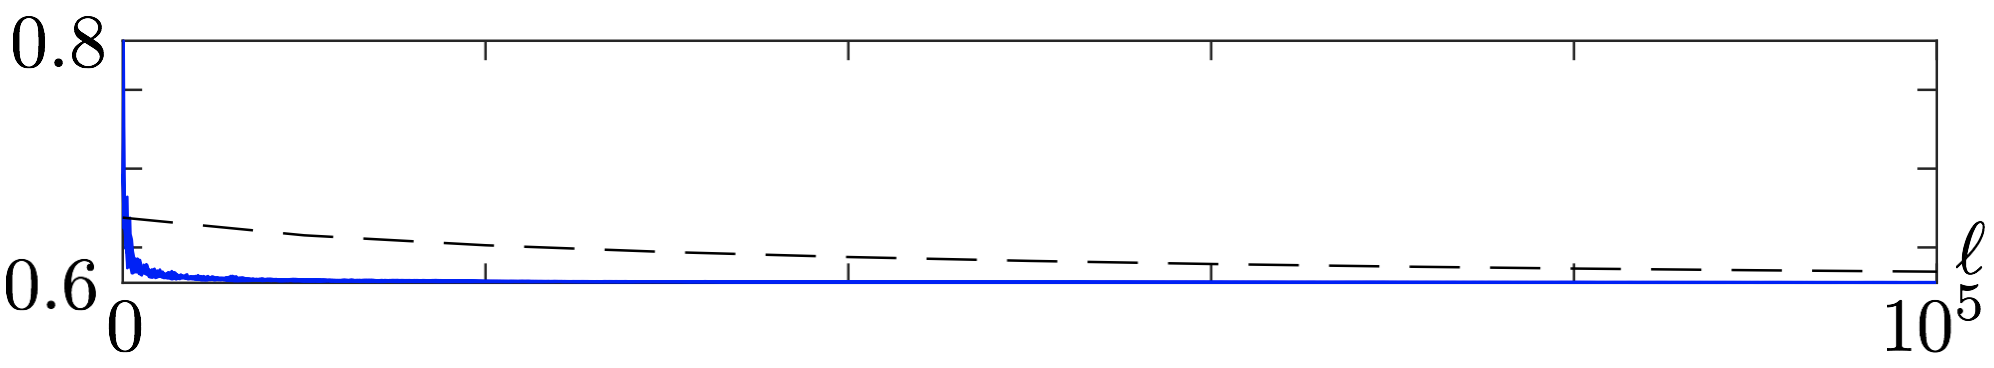
\includegraphics[width=.45\linewidth]{ml/sgd/error-sgd-1} &
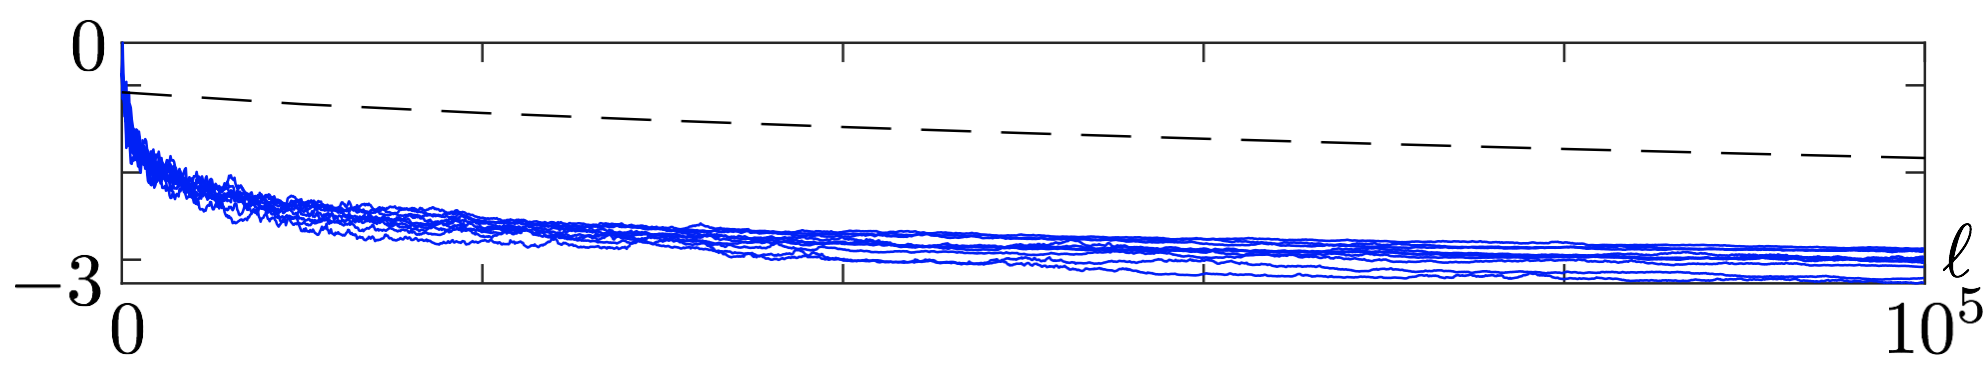
\includegraphics[width=.45\linewidth]{ml/sgd/error-sgd-2} \\
$f(x_k)$ & $\log_{10}(f(x_k)-f(x^\star))$ 
\end{tabular}
\caption{\label{fig-sgd}
Evolution of the error of the SGD for logistic classification (dashed line shows BGD).
}
\end{figure}




%%%%%%%%%%%%%%%%%%%%%%%%%%%%%%%%%%%%%%%%%%%%%%%%%%%%%%%%
\subsection{Stochastic Gradient Descent with Averaging (SGA)}
\label{sec-sga}

Stochastic gradient descent is slow because of the fast decay of
$\tau_k$ toward zero.
%
To improve somehow the convergence speed, it is possible to average the past
iterate, i.e. run a ``classical" SGD on auxiliary variables $( \tilde x_k)_k$
\eq{
	 \iit{\tilde x} = \tilde x_k - \tau_k \nabla f_{i(k)}(\tilde x_k)
}
and output as estimated weight vector the Cesaro average
\eq{
	x_k \eqdef \frac{1}{k} \sum_{\ell=1}^k \tilde x_{\ell}.
}
This defines the Stochastic Gradient Descent with Averaging (SGA)
algorithm.

Note that it is possible to avoid explicitly storing all the iterates by simply
updating a running average as follow
\eq{
	x_{k+1} = \frac{1}{k} \tilde x_k +  \frac{k-1}{k} x_k. 
}


In this case, a typical choice of decay is rather of the form 
\eq{
	\tau_k \eqdef \frac{\tau_0}{1 + \sqrt{k/k_0}}.
}
Notice that the step size now goes much slower to 0, at rate $k^{-1/2}$.


Typically, because the averaging stabilizes the iterates, the choice of
$(k_0,\tau_0)$ is less important than for SGD. 

% <https://arxiv.org/pdf/1303.6149.pdf 

Bach proves that for logistic classification, 
it leads to a faster convergence (the constant involved are
smaller) than SGD, since 
on contrast to SGD, SGA is adaptive to the local strong convexity of $E$.



%%%%%%%%%%%%%%%%%%%%%%%%%%%%%%%%%%%%%%%%%%%%%%%%%%%%%%%%
\subsection{Stochastic Averaged Gradient Descent (SAG)}

% https://arxiv.org/pdf/1309.2388
For problem size $n$ where the dataset (of size $n \times p$) can
fully fit into memory, it is possible to further improve the SGA method
by bookkeeping the previous gradients. This gives rise to the 
Stochastic Averaged Gradient Descent (SAG) algorithm.

We store all the previously computed gradients in $(G^i)_{i=1}^n$,
which necessitates $O(n \times p)$ memory. 
The iterates are defined by using a proxy $g$ for the batch gradient,
which is progressively enhanced during the iterates.

The algorithm reads
\eq{
	x_{k+1} = x_k - \tau g
	\qwhereq
	\choice{
	h \leftarrow \nabla f_{i(k)}(\tilde x_k), \\
	g  \leftarrow g - G^{i(k)} + h,   \\
	G^{i(k)} \leftarrow h.
	}
}
Note that in contrast to SGD and SGA, this method uses a fixed step
size $\tau$. Similarly to the BGD, in order to ensure convergence, 
the step size $\tau$ should be of the order of $1/L$
where $L$ is the Lipschitz constant of $f$.

This algorithm improves over SGA and SGD
since it has a convergence rate of $O(1/k)$ as does BGD. 
Furthermore, in the presence of strong convexity (for instance when $X$ is
injective for logistic classification), it has a linear convergence rate, 
i.e. 
 \eq{
	\EE( f(x_k) ) - f(x^\star) = O\pa{ \rho^k },
}
for some $0 < \rho < 1$. 

Note that this improvement over SGD and SGA is made possible only because
SAG explicitly uses the fact that $n$ is finite (while SGD and SGA can
be extended to infinite $n$ and more general minimization of
expectations~\eqref{eq-min-int}).

Figure~\ref{fig-compariso-sgd} shows a comparison of SGD, SGA and SAG.

\begin{figure}
\centering
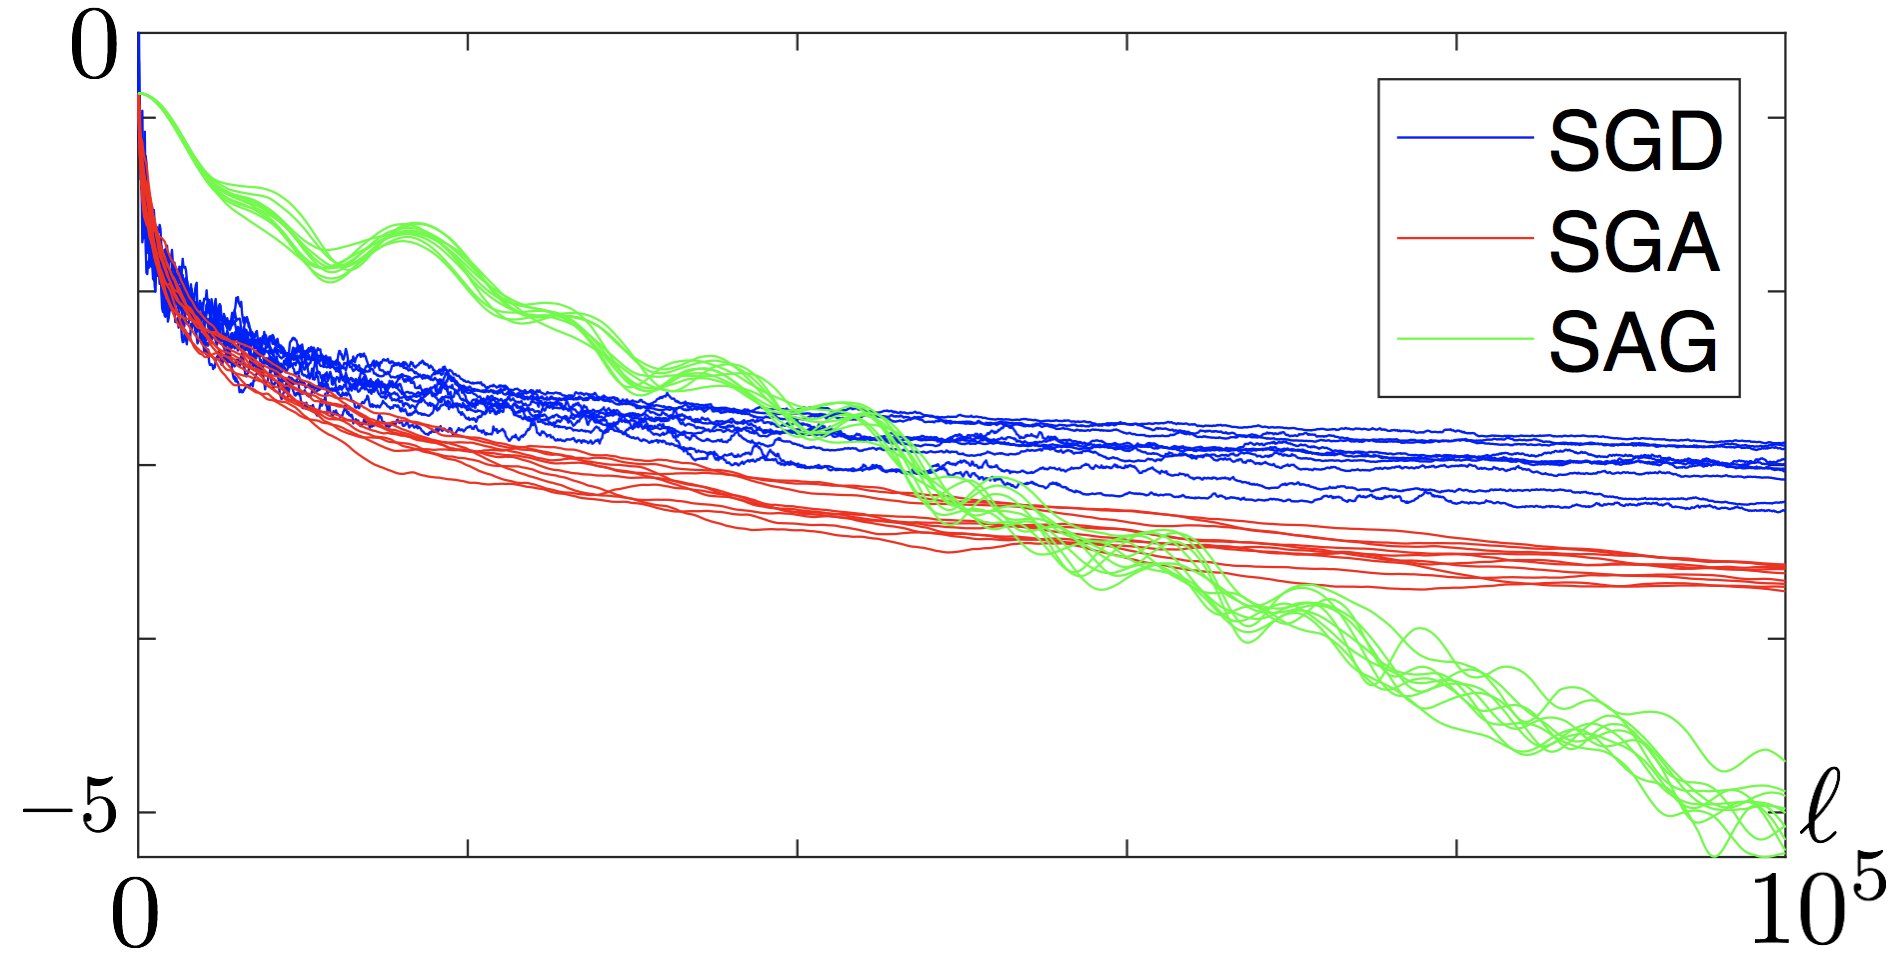
\includegraphics[width=.5\linewidth]{ml/sgd/sg-comparison}
\caption{\label{fig-compariso-sgd}
Evolution of $\log_{10}(f(x_k)-f(x^\star))$ for SGD, SGA and SAG.
}
\end{figure}



